
\tikzstyle{MStyle}=[fill=blue!30]
\tikzstyle{TStyle}=[fill=red!30]
\tikzstyle{SStyle}=[fill=green!30]

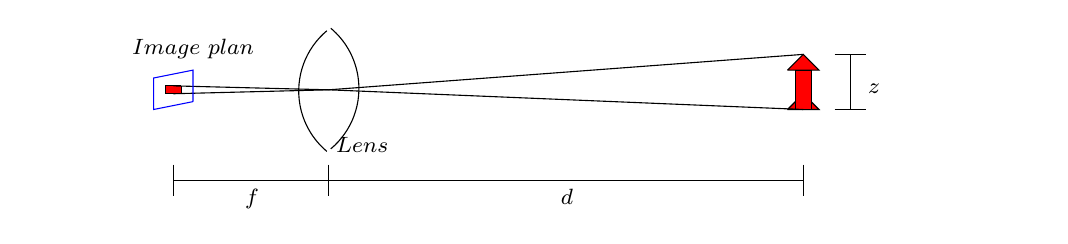
\begin{tikzpicture}[every node/.style={draw, text centered ,rounded corners, minimum width=4cm,text width=4cm}]
\footnotesize
%----------------------------------------------------------
	% Vertices of the triangle
	%------------------------------------------------------
	\coordinate[] (A) at (0.25,-1.4);
%	\coordinate[label=$B$]  (B) at (8,2); 
	\coordinate[] (RocTop) at (8,-0.8);
	\coordinate[] (RocBot) at (8,-1.5);
	\coordinate[] (RangTR) at (0.25,-1);
	\coordinate[] (RangTL) at (-0.25,-1.1);
	\coordinate[] (RangBL) at (-0.25,-1.5);	
	\coordinate[label=below:$~~~~~~~~Lens$] (ARC) at (2,-1.75);
	
	\coordinate[label=below:$Image~plan$]  (MD) at (0.25,-0.5);
	\coordinate[label=below:$f$]  (f) at (1,-2.4);
	\coordinate[label=below:$d$]  (d) at (5,-2.4);
	\coordinate[label=$z$]  (z) at (8.9,-1.4);
	
	%Rocket
	%------------------------------------------------------
	\draw[fill=red] (7.8,-1) -- (8,-0.8) -- (8.2,-1) -- (7.8,-1);	
	\draw[fill=red] (7.8,-1.5) -- (8,-1.3) -- (8.2,-1.5) -- (7.8,-1.5);	
	\draw[fill=red] (7.9,-1) -- (8.1,-1) -- (8.1,-1.5) -- (7.9,-1.5) -- (7.9,-1);
	
	%On imageplan
	\draw[fill=red] (0.1,-1.2) -- (-0.1,-1.2) -- (-0.1,-1.3) -- (0.1,-1.3) -- (0.1,-1.2);	
	
	%Lines
	%------------------------------------------------------	
	\draw (2,-2) arc(-50:50:1);
	\draw (1.95,-0.5) arc(-50:50:-1);
	\draw[] (RocBot) -- (1.975,-1.25);
	\draw[] (RocTop) -- (1.975,-1.25);
	\draw[] (1.975,-1.25) -- (0,-1.2);
	\draw[] (1.975,-1.25) -- (0,-1.3);

	%Imageplan
	%------------------------------------------------------
	\draw[color=blue] (A) -- (RangTR) -- (RangTL) -- (RangBL) -- (A);
	
	%Measure Lines
	%------------------------------------------------------
	\draw (1.975,-2.2) -- (1.975,-2.6);	
	\draw (0,-2.2) -- (0,-2.6);	
	\draw (8,-2.2) -- (8,-2.6);	
	
	\draw (1.975,-2.4) -- (8,-2.4);	
	\draw (1.975,-2.4) -- (0,-2.4);
	
	\draw (8.4,-1.5) -- (8.8,-1.5);	
	\draw (8.4,-0.8) -- (8.8,-0.8);
	\draw (8.6,-1.5) -- (8.6,-0.8);	
	 
\end{tikzpicture}